\documentclass{llncs}
\usepackage[ngerman]{babel}
\usepackage[utf8]{inputenc}
\usepackage[T1]{fontenc}
\usepackage{amssymb}
\usepackage{graphicx}
\begin{document}
\pagestyle{headings}

\mainmatter

\title{Adaptive Gestenerkennung mit Variationsabschätzung für interaktive Systeme}

\titlerunning{Gestenerkennung}

\author{Maxim Boianetchii\inst{1} \and Marian Stein\inst{2}}

\authorrunning{Maxim Boianetchii,  Marian Stein}

\institute{Universität Rostock\\
\email{maxim.boianetchii@uni-rostock.de}
\and
Universität Rostock\\
\email{marian.stein@uni-rostock.de}}

\maketitle
\section{Einführung}
Dieser Artikel stellt eine Gestenerkennung / ein Adaptionssystem für die Mensch-Computer-Interaktion vor. Es beschreibt ein vorlagenbasiertes Erkennungsverfahren, das durch einen Anpassungsprozess, die Gestenvariation in Echtzeit verfolgt. Die wichtigsten Vorteile sind geschätzten Parameter und Erkennungsergebnisse. Die Technik wurde auf verschiedene Weisen in einer Benutzerstudie mit 3D Gesten im freien Raum ausgewertet. Hierbei wurde festgestellt, dass das Verfahren robust gegen Rauschen ist und erfolgreich sich an Variationsparameter anpasst. Dieses Verfahren führt die Erkennung genauso gut oder sogar besser als andere Methoden durch.

Die Gesten werden für verschiedenen Formen der Aktivitätserkennung verwendet. Es besteht ein Bedarf für aufwändige Interaktionsparadigmen, die auf Körperbewegungen oder greifbare Geräte und Schnittstellen basieren. Es gibt bereits Verfahren zur diskreten und kontinuierliche Gestenerkennung, die erfolgreich umgesetzt wurden. Diese Verfahren wurden entwickelt um die Geste in den meisten Fällen zu markieren. In diesem Experiment wird eine ganz neue Technik vorgeschlagen, die über Klassifikation hinausgeht, eine Bewegung kennzeichnet und die Möglichkeit bietet, innovative Interaktionsszenarien zu nutzen.
Die Benutzer müssen  ständig ihre Bewegungen anzupassen und sich zum Beispiel auf optische oder akustische Rückmeldung verlassen. Die Gesten, die erkannt werden, können in Vergleich zu Referenzgesten „verzerrt“ angezeigt werden.Ein robustes Erkennnungssystem muss in der Lage sein, sich an solche Änderungen anzupassen. Außerdem wäre es nützlich die Parameter der Geste während der Ausführung schrittweise zu schätzen. Dies ermöglicht dem System die Berücksichtigung von Schwankungen, die während der Bewegung und Aktualisierung des Bewegungsmodells auftreten,  wahrzunehmen. Derartige Parametrisierung  könnte direkt in der Gestaltung der Interaktion verwendet werden.
Caramiaux et al. \cite{Caramiaux2014} schlägt ein neues Gestenerkennungssystem vor, das in der Lage ist, in Echtzeit die berücksichtigte Bewegung und Variation inkrementell während der Durchführung wahrzunehmen und dem Nutzer Parameter zurückzuliefern. Es können verschiedene Gestenvariationen innerhalb der Geschwindigkeit, Amplitude oder Orientierung aufgenommen werden. Wichtig ist, dass diese Variationen kontinuierlich während der Ausführung der Gesten geschätzt werden können. Diese Methode ist ein Zustandsraummodel, in dem Variationen online geschätzt werden. Dazu braucht man einen Partikelfilter um kontinuierlich die Variation der Geste anzupassen.


\section{Ähnliche Arbeiten}
In diesem Abschnitt untersuchen wir Methoden die am meisten benutzt werden um Gesten, die als mehrdimensionale Zeitreihen für die Mensch-Computer-Interaktion vorgestellt sind, zu erkennen. Die mehrdimensionalen Zeitreihen stellen die Bahn eines Punktes auf einer Oberfläche oder in dem 3D-Raum dar. 
Rubine\cite{Rubine1991} schlägt ein geometrisches Abstandmaß basierend auf Beispielen von Einzeltakt-Gesten vor. Wobbrock et al.\cite{Wobbrock2007} schlagen eine einfache Template-basierte Methode vor, die Nutzung des euklidische Abstands nach einer Vorverarbeitungsstufe zur Berücksichtigung geometrischer Variationen (wie Skalierung und Rotation) und Drehzahlschwankungen ermöglicht.
[Gawrila und Davis\cite{Gawrila1995} und Liu et al.\cite{Liu2009} schlagen Dynamic Time Warping (DTW) vor, das erfordert die Speicherung des gesamten zeitlichen Struktur der Geste. Es gibt verschiedene Anwendungen, wie Gestensteuerung\cite[Merrill et al.]{Merrill2006} kommunikative Gestenfolgen \cite[Heloir et al. 2006]{Heloir2006}, und Abfragen auf Basis menschlicher Bewegung \cite[Forbes und Fiume 2005]{Forbes2005}. 
Statistische Methoden, wie das Hidden Markov Model (HMM) \cite[Rabiner 1989]{Rabiner1989}, das auf einer Wahrscheinlichkeitsinterpretation der Beobachtungen (Probegesten) basiert und zeitliche Trajektorie der Geste durch eine kompakte Darstellung modellieren kann. 
Variationen in der Geste werden zum größten Teil durch Methoden wie HMM, die umfassende Datenbanken verwenden, unter Berücksichtigung aller möglichen Variationen. 
 Wilson und Bobick\cite{Wilson1999} schlagen ein Modell vor, das die parametrische Änderungen in der Ausführung berücksichtigt.
In diesem Artikel wird gezeigt, dass ein adaptiver Ansatz mit einem ausgefahrenen Zustand Modell und einem anderen Decodierschema möglich ist.
Die von Caramiaux et al.\cite{Caramiaux2014} vorgeschlagene Methode, durch die Arbeit von Black und Jepson \cite[1998a]{BlackandJepson1998a} inspiriert, basiert auf dem Kondensationsalgorithmus \cite[Isard und Blake 1998]{IsardandBlake1998} für die Anerkennung der raumzeitlichen Vorlagegesten, der die Umsetzung für die Verfolgung von Geschwindigkeit und Skalierungsänderung erlaubt.Caramiaux et al.\cite{Caramiaux2014} verallgemeinern den Ansatz von Black und Jepson [1998a] durch Schätzen nicht nur der Skalierung, sondern auch anderer Parameter, wie Rotation.


\section{Interaktionsprinzipien}
Caramiaux et al.\cite{Caramiaux2014} präsentieren Interaktionsprinzipien, die wichtig für Zielanwendungen wie Ton Manipulation oder Visual Processing in Kontexten wie Spiele, interaktive Kunst oder Rehabilitation sind. Ihr Interaktionsmodel beinhaltet zwei Arten von Kontrolle: die Ausführung einer Geste und wie sie durchgeführt wird. Die Körperbewegungen werden von einem Bewegungserfassungsgerät erfasst. Der Algorithmus ist in der Lage die Geste zu erkennen, an ihre  Variation und Veränderungen anzupassen und die Variationsparameter mit Berücksichtigung der zuvor gelernten Vorlagen zurückliefern. Die Erkennung und Adaption werden in Echtzeit durchgeführt. Die Ausgabe des Algorithmus wird fortlaufend aktualisiert. Der Modelausgang hat zwei Komponenten:  einen Index für die erkannten Gesten und einen Vektor für kontinuierliche Werte der Schätzung der Variation. Zur Erleichterung der schnellen Testsitzungen und um das Lernverfahren so leicht wie möglich zu machen, wird von System nur eine einzige Schablone zum Definieren einer bestimmten Geste Klasse erforderlich.

\section{Zugrunde liegendes Modell}
Wir definieren Gesten so, dass eine Geste ist eine Körpergliedbewegung ist, die durch eine zeitliche Reihe einer festen Anzahl von Parametern vertreten wird. Für eine eingegebene Geste wählt der Erkennungsschritt die beste Übereinstimmung aus einer Menge von Vorlagen aus.
\subsection{ Kontinuierliche Zustandsmodell}
Das Modell kann mit folgendem dynamischen System formuliert werden:
\begin{equation}
\left\{\begin{array}{l}
x_k = f_{TR} (x_{k-1}, v_{k-1}) \\
z_k = f_{OB} (x_k, w_k; g) \\
\end{array}\right.
\end{equation} 										
wobei k diskreter Zeitpunkt ist.
\begin{itemize}
	\item $x_k$ ist ein Vektor, der den Systemzustand und Zustand der Elemente unterschiedlichen Geste Eigenschaften vorstellt
	\item $f_{TR}$ ist eine Funktion, die die Entwicklung des Systemzustands regelt
	\item $v_k$ ist eine Rauschsequenz
	\item $f_{OB}$ ist eine Funktion, die die Beobachtungen $z_k$ erzeugt, je über den Systemzustand $x_k$ und Messrauschsequenz $w_k$ und eine Vorlage Geste $g$.
\end{itemize}
Das Problem wird als ein Verfolgungsproblem formuliert.

\subsection{ Zustandsraummodel}
Der Zustand des Systems besteht aus unterschiedlichen Merkmalen und Eigenschaften von Gesten, die über eine lange Zeit geschätzt werden. Der Zustandsraum umfasst die Merkmale, die online bewertet können und folglich als Dauerleistungen während der Interaktion verwendet werden. Die Funktionen werden in jedem Zeitschritt aktualisiert.

\subsection{ Zustandsübergang}

In diesem Modell ist die Zustandsübergangsfunktion $f_{TR}$ linear und durch Matrix $A$ gegeben und als Gauß-Verteilung modelliert: 

\begin{equation}
\left.\begin{array}{l}
 p(X_k|X_{k-1}) =  N(X_k|A_{X_{k-1}},\sum )\\\\ 
		\sum   = diag(\sigma_1...\sigma_D)             \\
		\\
\end{array}\right.		
\end{equation}

Durch Festlegen einer Beziehung zwischen Phase und Geschwindigkeit der Geste wurde eine Einschränkung in Form einer Bewegungsgleichung erster Ordnung gemacht. 
\begin{equation}
\left.\begin{array}{l}
p_k=p_{k-1} + V_k/T + N(0,\sigma_1)	
\end{array}\right.		
\end{equation}					
\\
wobei $T$ Lange der Vorlage und $\sigma_1$ das erste Element in der Diagonale der$ \sum$. Diese Einschränkung kann durch Einstellen der ersten Zeile der Matrix A in $ (1  \frac{1}{T}  0 ...0) $ berücksichtigt werden. Die andere Bedingungen werden in der ersten Zeile auf Null gesetzt.
Die Übergangsparameter spielen eine wichtige Rolle für die Anpassung. Sie regeln die Dynamik  der Veränderungsschätzung: die Geschwindigkeit der Annäherung an die genaue Schätzung und die Präzision der Schätzung.

\subsection{Beobachtungsfunktion} 
Die Beobachtungsfunktion wertet die Genauigkeit der Zustandsschätzung gemäß Eingangsbeobachtung und der Vorlage. Parameter der Beobachtungsfunktion legen fest, wie stark die Methode abweicht.
\begin{equation}
\left.\begin{array}{l}
S_t(Z_k|f(X_k, g(p_k)),\sum,v) = C(\sum, v)(1+ \frac{d^2(Z_k, f(X_k,g)}{v}  )^{-\frac{v+K}{2}}		
\\
\end{array}\right.		
\end{equation}	
\\
wo:
\begin{equation}
\left.\begin{array}{l}
C(\sum, v) =  \frac{\Gamma(v/2+K/2)  }{\Gamma(v/2) }\frac{|\sum|^{-1/2}}{(v \pi)^{K/2}}
\end{array}\right.
\end{equation}
wobei $f (X_k, g)$ eine Funktion des Templates $g$ und den Zustandswert bei $k$ ist. $ f (X_k, g)$ passt sich die erwartete Vorlage Probe $g$ (Stück), da die Phase $p_k$ bei $k$ gegeben ist. Der Abstand $d$ zwischen der angepassten Vorlageprobe und dem eingehenden Beobachtung ist gegeben durch:
\begin{equation}
\left.\begin{array}{l}
d(Z_k, f(X_k, g)) = \sqrt{[Z_k - f(X_k, g)]^T \sum^{-1} [Z_k - f(X_k,g)]}.			
\end{array}\right.		
\end{equation}	

\subsection{ Inferenz und Implementation}
Inferenz ist die Echtzeitschätzung der Zustandswerte. Hier wird die  Zustandsprobe aus einer einfacheren Verteilung entnommen und entsprechend ihrer Bedeutung bei der Schätzung der "wahren" Verteilung gewichtet. Bei jedem Schritt $k$ stellt ein Teilchen $x^i_k$ einen möglichen Wert des Zustandsraums, der von seiner Wahrscheinlichkeit $w^i _k$ gewichtet wird. Der Erwartungswert der Merkmale, zu dem Zeitpunkt $k$ ist:
\\
\\
$
\hat{X}_k = \sum_{i=1}^{N_s}{w^i_k} X^i_k
$
\\
\\
wobei $ N_s$ die Anzahl der Teilchen bezeichnet. Abgeleitete Merkmalswerte $\hat{X}_k$ bilden den Anpassungsprozess, seit dem Zeitpunkt $k$. Es werden die Variationswerte beurteilt, die als Zustandsvariablen definiert sind. 

\subsection{Bearbeitung der Anerkennung}
Schließlich wird das Modell erweitert, um Erkennung zu behandeln, indem mehrere Schablonen in Betracht gezogen werden. Der Zustandsraum wird geändert, um die wahrscheinlichste Schablone zusätzlich zu den variierenden Gesteneigenschaften zu schätzen.
Betrachtet werden M Vorlagen jeweiliger Länge $L_1 ... L_M$ bezeichnet durch $g^1 ... G^M$. Bei der Initialisierung, wird jedem Zustandspartikel $x^i_k$ eine Geste mit Index zwischen $1 ... M (m_k bezeichnet)$ zugeordnet, auf der Grundlage einer Anfangsverteilung. Im allgemeinen wird eine gleichmäßige Verteilung gewählt. Dies erweitert die Zustandskonfiguration angewandt auf jedes Partikel wie folgt: 
\begin{equation}
\left.\begin{array}{l}
X^i_k =
 $$  \left(\begin{array}{crl}
 X^i_k (1)\\		
				.\\
				.\\
				.\\
			X^i_k (D)\\
				m_k\\ 
				
				\end{array}\right)
		$$ \in \mathbb{R}^D \times \mathbb{N}						
\end{array}\right.		
\end{equation}	

Die Übergangswahrscheinlichkeit wird wie folgt angepasst:
\begin{equation}
\left.\begin{array}{l}				
p(X^i_k|X^i_(k-1) = N(X^i-k|A_(X^i_(k-1)), \sum)\\
			\sum =diag(\phi_1 ... \phi_D 0).								
\end{array}\right.		
\end{equation}				
			
Durch Summieren der Gewichte $W^i_k$  der zugehörigen Gestenindizes der Partikel, ist es einfach, die Wahrscheinlichkeit jeder Geste zu berechnen:

$p(g^i_k|g^m_k) =\sum_{j\in J}^{} w^j_k,  \forall l \in [1,M], \forall m \in [1,M], m \neq l
$
wo:
 \begin{equation}
 \left.\begin{array}{l}	
J = {j \in [1,N_s]/ X^j_k (D+1) = l}.									
\end{array}\right.		
\end{equation}	
\section{Erkennung von realen 2D-Gesten}
Um die Gestenauswertung zu evaluieren, wurde die Gestendatenbank von Wobbrock et al.\cite{Wobbrock2007} verwendet. Diese enthält Daten von 16 Stiftgesten, die von zehn Teilnehmern in drei verschiedenen Geschwindigkeiten jeweils zehn mal aufgenommen wurden. Für die Versuche wurden pro Geste zufällig aus den Daten eines Teilnehmers jeweils ein Trainings- und ein anderer Testdatensatz ausgewählt. Insgesamt wurden 4 verschiedene Tests durchgeführt, die jeweils 100 Mal wiederholt wurden:
\begin{enumerate}
\item Gleiche Testbedingungen, wie sie von Wobbrock\cite{Wobbrock2007} verwendet wurden.
\item Einfluss von geänderten Verteilungsparametern.
\item Verwendung von Trainings- und Testdaten mit unterschiedlichen Geschwindigkeiten.
\item Genauigkeit der Erkennung von Gesten, während sie noch nicht abgeschlossen sind.
\end{enumerate}
Bei allen Tests außer 3. wurden Trainings- und Testdaten mit der gleichen Geschwindigkeit gewählt.
Da der von Caramiaux\cite{Caramiaux2014} beschriebene Gesture Variance Follower(GVF) auch Veränderungen in den Gesten erkennen und ausgeben soll, ergibt sich für diese Tests ein Zustandsraum $x_k$, der aus der Phase $p_k$, der Geschwindigkeit $v_k$, der Skalierung $s_k$ und dem Drehwinkel $\alpha_k$ besteht.

\subsection{Erkennung von Beispielen gleicher Geschwindigkeit}
Im ersten Test wurde die durchschnittliche Erkennungsrate sowie die Standartabweichung von GVF mit den erreichten Werten von \$1 Recognizer\cite{Wobbrock2007}, DTW und GF verglichen. 
Im Vergleich zu dem Gesture Follower(GF) erreicht GVF eine bessere Erkennungsrate ($98,11 \%$ gegenüber $95,78\%$), was sich darauf zurückführen lässt, dass GVF sich an Skalierung und Drehung anpasst.
Auch im Vergleich mit den beiden Offline-Methoden erreicht GVF leicht bessere Erkennungsraten ($98,11\%$ gegenüber $97,27\%$ bzw. $97,86\%$).

\subsection{Einfluss der Verteilungparameter auf die Erkennung}

\begin{figure}
\centering
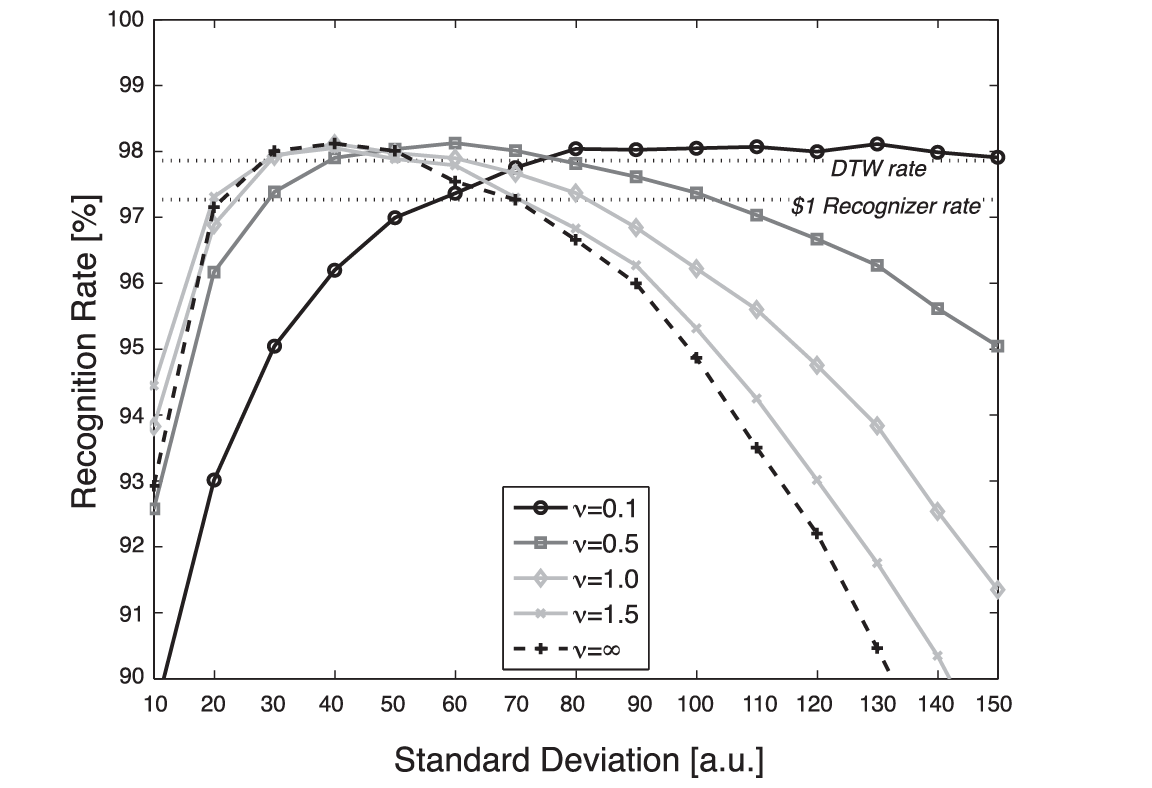
\includegraphics[width=0.7\linewidth]{../Bilder/Fig4}
\caption{Einfluss des Parameters $v$ und der Standardabweichung auf die Erkennungsrate}
\label{fig:Fig}
\end{figure}

Im zweiten Test wurde der Einfluss der Standartabweichung $\sigma$ und der Parameter $v$ der Student'schen t-Verteilung auf die Erkennungsrate untersucht. Untersucht wurden dabei für $\sigma$ in Zehnerschritten Werte von 10 bis 150 und für $v$ die Werte $0.5$, $1$, $1.5$ und $\infty$ (hier entspricht die Verteilung einer Gaussverteilung).

Die Ergebnisse sind in Abbildung \ref{fig:Fig} zusammen mit den Erkennungsraten der beiden Offline-Methoden dargestellt.


Hier sind zwei Beobachtungen festzustellen. Erstens, dass die Erkennungsrate die Beste ist für beschränkte $\sigma$ und $v$. Zweitens, dass die Verwendung einer Student'schen t-Verteilung anstatt einer Gaussverteilung den Vorteil hat, dass die Erkennungsrate wesentlich weniger von $\sigma$ abhängt.

\subsection{Erkennung von Beispielen verschiedener Geschwindigkeit}
Im dritten Test wurden die Erkennungsraten von GVF mit denen des \$1 Recognizers verglichen. Diesmal wurden allerdings die Vorlage und die Testgeste aus verschiedenen Geschwindigkeitsgruppen verwendet. Tabelle Y zeigt die Erkennungsraten der unterschielichen Kombinationsmöglichkeiten. Es wird deutlich, dass insgesamt die durchschnittliche Erkennungsrate beider Algorithmen vergleichbar ist ($94,6\%$ gegenüber $94,8\%$). Ebenso fällt auf, dass die schlechtesten Ergebnisse erreicht werden, wenn Vorlage und Testgeste  entgegengesetzte Geschwindigkeiten haben, mit Genaunigkeiten von $88,3\%$ bzw. $85,9\%$.

\subsection{Früherkennung der Gesten}
Zuletzt wurde die Erkennung der Gesten untersucht, während sie ausgeführt werden. In Graph Z sind die Früherkennungsraten von GVF und GF in Abhängigkeit vom Fortschritt der Geste dargestellt. Es wird deutlich, dass GVF über den ganzen Messbereich bessere Erkennungsraten erreicht als GF. So erzielt GVF im Schnitt bereits nach $10\%$ der Geste eine Genauigkeit $67\%$ und erreicht bereits nach $40\%$ Fortschritt $90\%$ Genauigkeit.

\subsection{Ergebnisse der Versuche mit realen Daten}
In den Versuchen hat sich gezeigt, dass GVF in der Erkennung von Gesten gleich gut bis besser ist als andere aktuelle Erkennungsmethoden. Darüber hinaus wurde deutlich, dass die im GVF verwendete Student'sche t-Verteilung gegenüber der im GF verwendeten Gaussverteilung weniger auf eine gute Abschätzung von $\sigma$ angewiesen ist. Somit ist diese Methode besser in Anwendungsfällen verwendbar, in denen wenig Trainingsdaten zur Verfügung stehen, und somit $\sigma$ schlecht abgeschätzt werden kann. Eine Verbesserung gegenüber bisher üblichen Methoden stellt der GVF auch dadurch dar, dass bereits während der Gestenausführung Ergebnisse geliefert werden, und die Früherkennung gut genug funktioniert, dass schon nach $10\%$ der Geste Erkennungsgenauigkeiten von über $60\%$ erreicht werden.

\section{Abschätzung der Varianz anhand synthetischer Daten}
Um die Anpassung an Varianz der Gesten auszuwerten, wurden synthetische Daten verwendet, da menschliche Eingaben keine exakten Werte für die Varianzparameter liefern würden, mit denen die Ergebnisse des GVF verglichen werden könnten. Es wurden zwei Fälle betrachtet: Im ersten Fall wurde nur die Phase und Skalierung der Gesten variiert, im zweiten Fall zusätzlich auch die Rotation. Für die Generierung der Daten wurde eine Viviani-Kurve verwendet:
\begin{equation}
C(t)=\left\{\begin{array}{l}
x(t)=a(1+\cos(t))\\
y(t)=a\sin(t)\\
z(t)=2a\sin(t/2)\\
\end{array}\right.
\end{equation} 

\subsection{Auswertung der Phasenabschätzung}
\begin{figure}
\centering
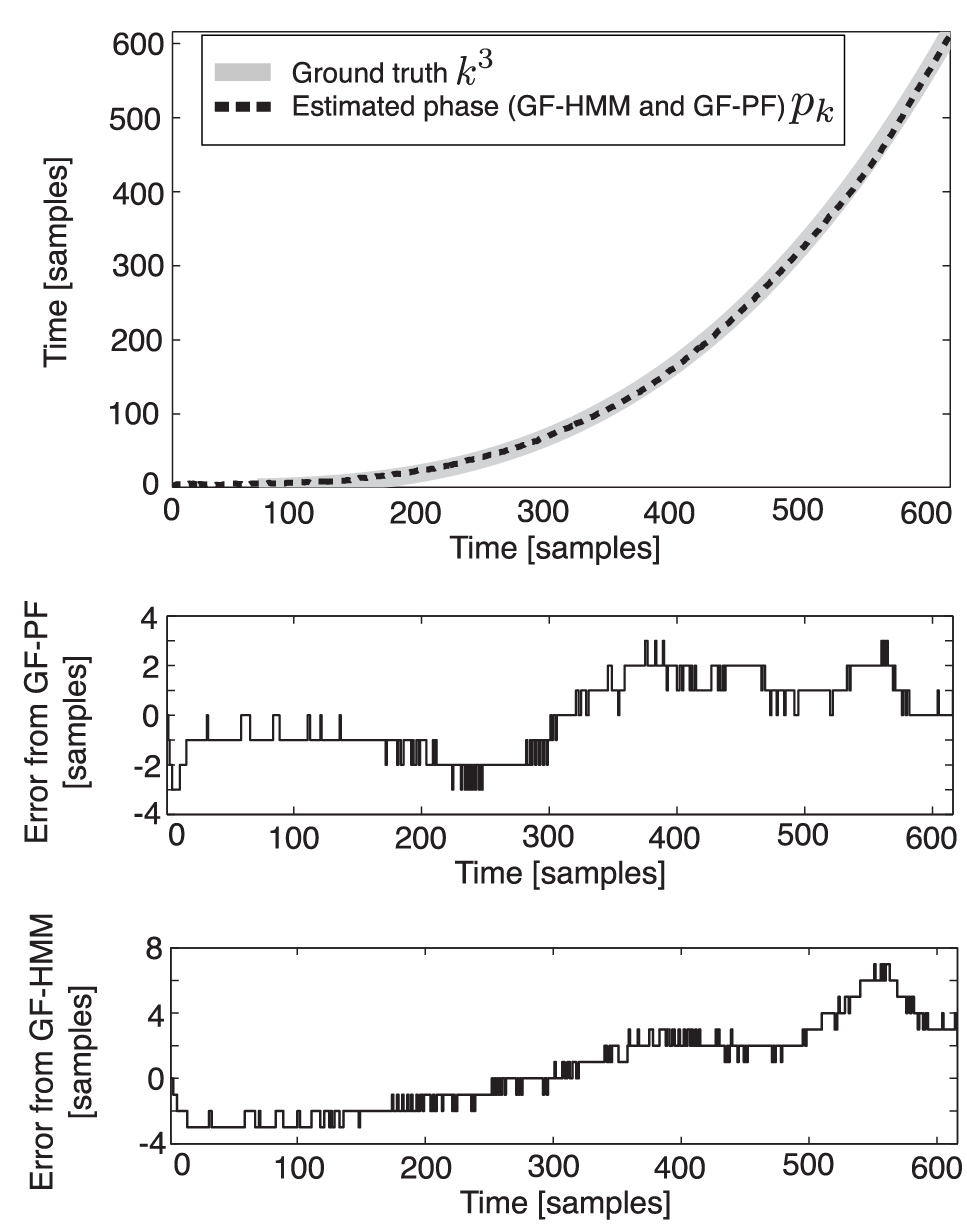
\includegraphics[width=0.7\linewidth]{../Bilder/Fig6}
\caption{}
\label{fig:Fig6}
\end{figure}
Für diesen Fall wurde als Vorlage eine lineare Abstastung der Viviani-Kurve, und als Testdaten eine kubische Abtastung( $ t \rightarrow t^3 $ ) zu der ein gleichmäßig verteiltes Rauschen hinzugefügt wurde, verwendet. Der Zustandsraum ist hier dreidimensional, bestehend aus der Phase $ p_k \in [0,1] $, der Geschwindigkeit $v_k \in \mathbb{R}$ und der Skalierung $s_k \in \mathbb{R}$, wobei $v_k$ und $s_k$ so normalisiert sind, dass ein Wert von 1 jeweils der Geschwindigkeit bzw. Skalierung der Vorlage entspricht. Um einen Vergleich zu GF machen zu können, wurde $v \rightarrow \infty$ gewählt.

Im Vergleich erreichten beide Verfahren gute Abschätzungen mit durchschnittlichen Fehlern von 1,3 Abtastungen beim GVF, bzw. 2,3 Abtastungen beim GF.

Weiter wurde der Einfluss von $\sigma$ auf die Abschätzungen untersucht. Die Ergebnisse sind in Abbildung \ref{fig:Fig6} dargestellt. Für alle getesteten Werte für $\sigma$ lieferte GVF bessere Abschätzungen als GF, obwohl GF eine genauere Inferenztechnik verwendet. Dies liegt daran, dass GVF ein besseres kontinuierliches Modell verwendet, um die Daten wiederzuspiegeln, sowie an dem Zusammenhang zwischen Geschwindigkeit und Phase, welcher von GF ignoriert wird.

Ebenso stellte sich heraus, dass GVF bessere Abschätzungen in Abhängigkeit von der Stärke des Rauschens liefert, als GF.

\subsection{Auswertung der Rotationsabschätzung}
\begin{figure}
\centering
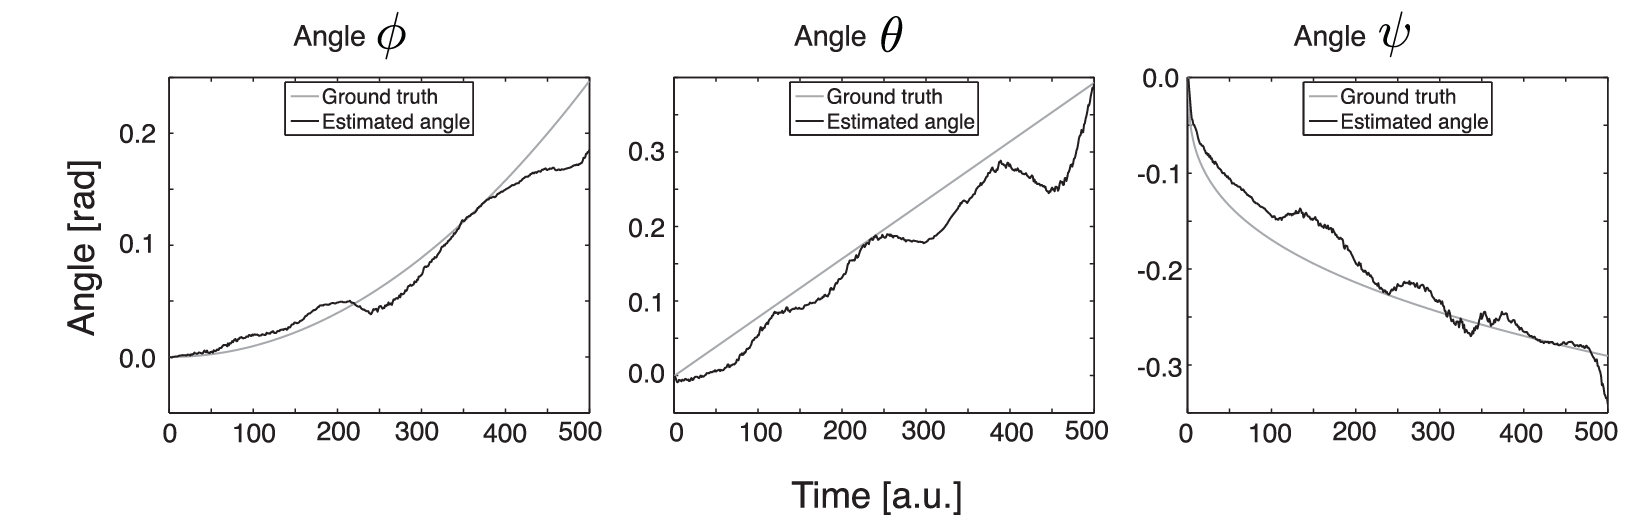
\includegraphics[width=0.7\linewidth]{../Bilder/Fig8}
\caption{}
\label{fig:Fig8}
\end{figure}
Für diesen Versuch wurde die Rotation der Geste mit der Zeit variiert. Die Drehwinkel $\phi$, $\theta$ und $\psi$ für die Drehung entlang der $x$, $y$ und $z$-Achse wurden pro Zeitschritt berechnet durch:
\begin{equation}
\begin{array}{rcl}
\phi(t) & = & t^2\\
\theta(t) & = & t\\
\psi(t) & = & -t^{1/3}
\end{array}
\end{equation}
Der Zustandsraum ist hier entsprechend 5-dimensional, bestehend aus $p_k$, $v_k$, $\phi_k$, $\theta_k$ und $\psi_k$. Es wurden die gleichen Tests durchgeführt wie bei der Phasenabschätzung.
Es stellt sich heraus, dass $\sigma$ wenig Einfluss auf die Genauigkeit der Abschätzung hat, aber dass bei niedrigen Werten für $\sigma$ die Fehlerrate stärker schwankt als bei großen Werten.

\subsection{Ergebnisse der Auswertung synthetischer Daten}
In beiden Experimenten wurde deutlich, dass $\sigma$ wenig Einfluss auf die Abschätzung hat. Daher ist der Algorithmus auch anwendbar, wenn es nur sehr wenig Trainingsdaten gibt. Ebenso stellte sich heraus, dass die Phasenabschätzung bei festem Rauschen und $\sigma$ mit einem Durchschnittsfehler von 2,3 Abtastungen sehr genau ist. Zuletzt hat die Stärke des Rauschens einen zu erwartenden Einfluss auf die Abschätzung, wobei sie noch gut genug bleibt, dass der Algorithmus auch bei signifikantem Rauschen verwendet werden kann.

\section{Nutzerstudie}
\subsection{Durchgeführte Experimente}
\begin{figure}
\centering
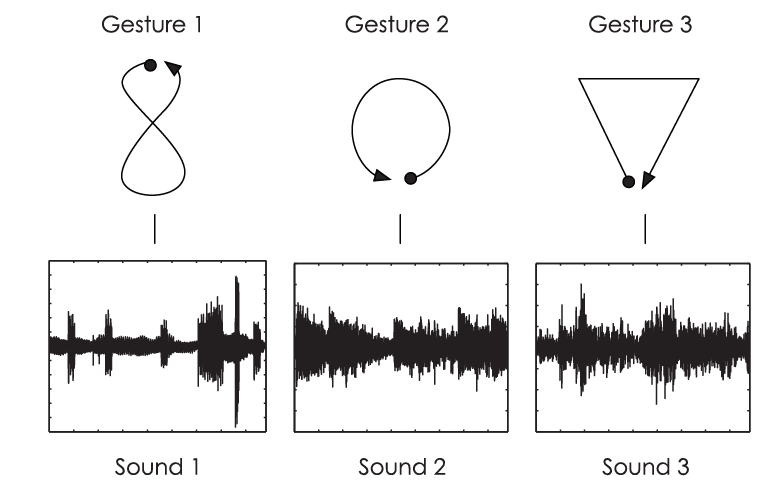
\includegraphics[width=0.7\linewidth]{../Bilder/Fig10}
\caption{Die von den Teilnehmern durchgeführten Gesten mit den dazugehörigen Tönen}
\label{fig:Fig10}
\end{figure}
Es wurde eine Nutzerstudie durchgeführt, um die Einbindung von GVF in reale Anwendungen zu untersuchen. Hierfür wurde eine Anwendung entwickelt, wo eine Gestenausführung die Wiedergabe eines vordefinierten Tons hervorruft, welcher durch Variationen in der Geste verändert wurde. Hierbei wird die Früherkennung des GVF verwendet, um den Ton abzuspielen, sobald die Wahrscheinlichkeit der Erkennung über 50\% beträgt. Ab dann werden für den Rest der Geste die Abschätzung der Varianzen für die Manipulation des Tons verwendet. Hierbei sorgt eine schnellere/langsamere Ausführung der Geste für eine schnellere/langsamere Wiedergabe des Tons, größere/kleinere Gesten sorgen für eine lautere/leisere Wiedergabe und eine Drehung der Geste regelt die Cut-Off-Frequenz eines Hochpassfilters. Den Teilnehmern werden 7 Aufgaben gestellt, die alle daraus bestehen, einen bestimmten Ton abzuspielen, und ihn dann zu manipulieren. Hierbei ist zu beachten, dass Aufgabe 1 nur das Abspielen eines Tons, Aufgabe 2-4 eine globale Änderung eines Aspekts, Aufgabe 5 eine kontinuierliche Änderung eines Aspekts und Aufgabe 6 und 7 die globale Änderung zweier Aspekte beinhalten. Die Gesten werden von einem infrarotbasiertem System aufgenommen, welches Fingerbewegungen im freien Raum misst. Die Studie wurde mit 10 Teilnehmern durchgeführt, die jede der 3 Gesten 3 Mal pro Aufgabe durchführten. Somit ergeben sich 630 Datensätze. Jede aufgenommene Geste sowie der zugehörige wiedergegebene Ton wurden im Nachhinein analysiert, um die Abschätzung des Algorithmus auszuwerten.



Zunächst wurde die Erkennungsrate allgemein untersucht. Insgesamt wurden nur 17 Gesten nicht erkannt, es ergibt sich somit eine Erkennungsgenauigkeit von $97,3\%$. Anschließend wurde die Früherkennung der Gesten untersucht. Hierbei galt eine Geste als erkannt, sobald die Erkennungswarscheinlichkeit größer als $50\%$ ist. Im Durchschnitt wurde eine Geste nach $12,6\%$ der Durchführung erkannt.

\subsection{Anpassung einer Eigenschaft}
In den Aufgaben 2 bis 4 wurden die Teilnehmer beauftragt, eine Eigenschaft(Lautstärke, Geschwindigkeit und den Hochpassfilter) zu manipulieren. Die Ergebnisse wurden mithilfe eines Student'schen T-Tests mit den Ergebnissen von Aufgabe 1 verglichen.

\subsubsection{lauteres Abspielen des Tons}
\subsection{Beurteilung der Erkennungsgenauigkeit}
\begin{figure}
\centering
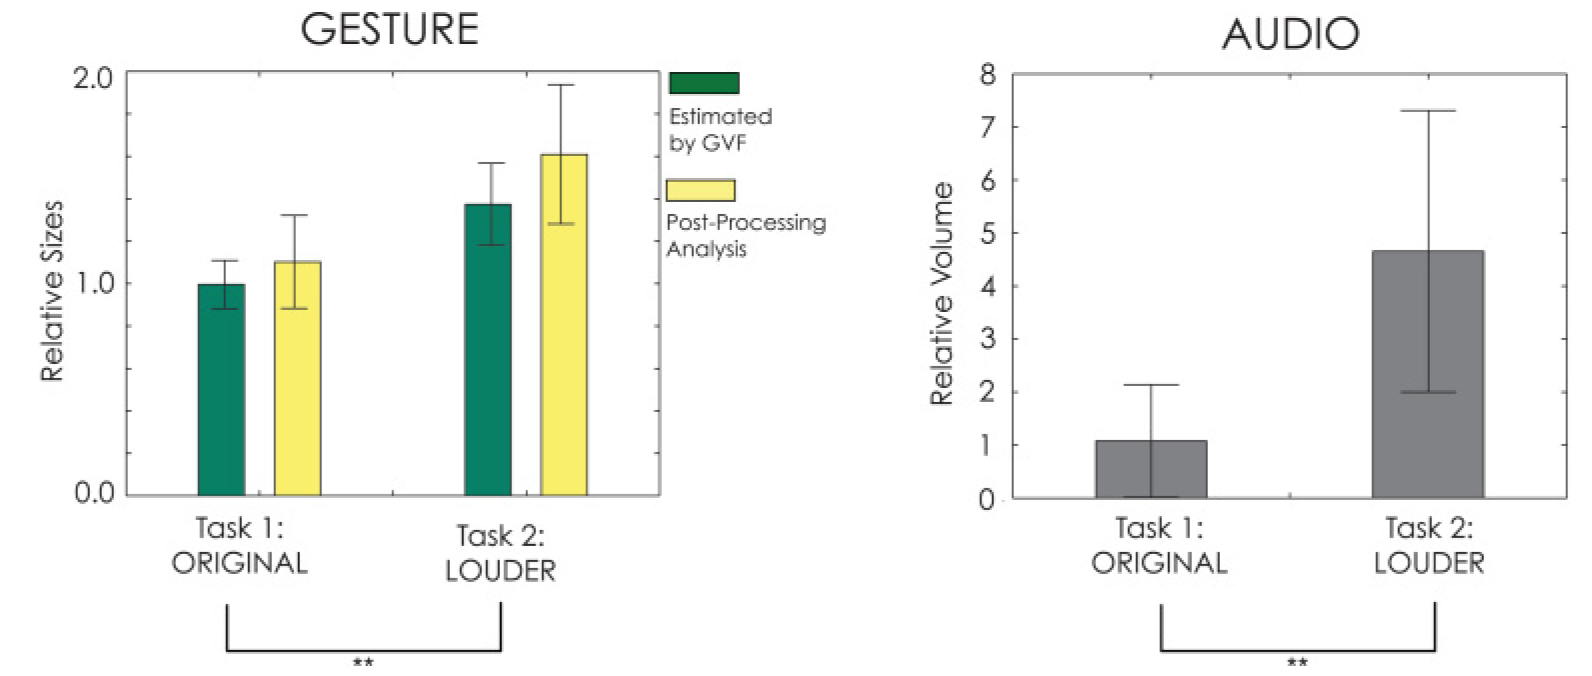
\includegraphics[width=0.7\linewidth]{../Bilder/Fig13}
\caption{Ergebnisse von Aufgabe 2 im Vergleich mit 1}
\label{fig:Fig13}
\end{figure}
In Abbildung \ref{fig:Fig13} wird deutlich, dass die Teilnehmer in der Lage waren, den Ton lauter als normal abzuspielen, da es signifikante Unterschiede der Mittelwerte von Aufgabe 1 und 2 gab. Ebenso zeigt sich, dass die Teilnehmer die Gesten wie gefordert größer ausgeführt haben, was von der Abschätzung auch wiedergespiegelt wurde.

\subsubsection{schnelleres Abspielen des Tons}
\begin{figure}
\centering
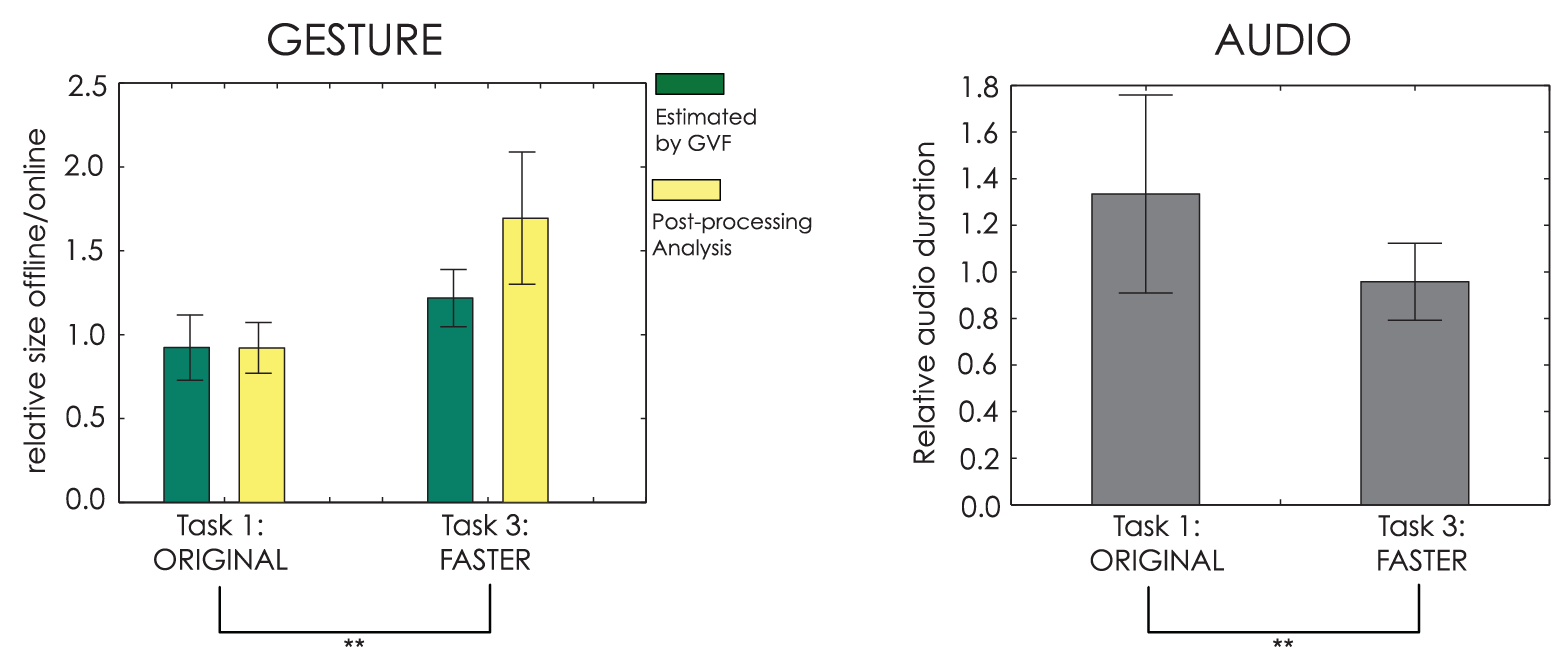
\includegraphics[width=0.7\linewidth]{../Bilder/Fig14}
\caption{Ergebnisse von Aufgabe 3 im Vergleich mit 1}
\label{fig:Fig14}
\end{figure}

Auch hier waren die Teilnehmer in der Lage, die Aufgabe zu erfüllen, da die durchschnittliche Länge eines Tons kürzer war als bei Aufgabe 1. Es ist aber zu bemerken, dass die Teilnehmer, wenn gebeten den Ton in Originalgeschwindigkeit abzuspielen, ihn etwas langsamer als das Original abspielten. Auch in diesem Versuch erkannte der Algorithmus eine Zunahme der Geschwindigkeit der Geste.

\subsubsection{Beeinflussung des Hochpassfilters}
\begin{figure}
\centering
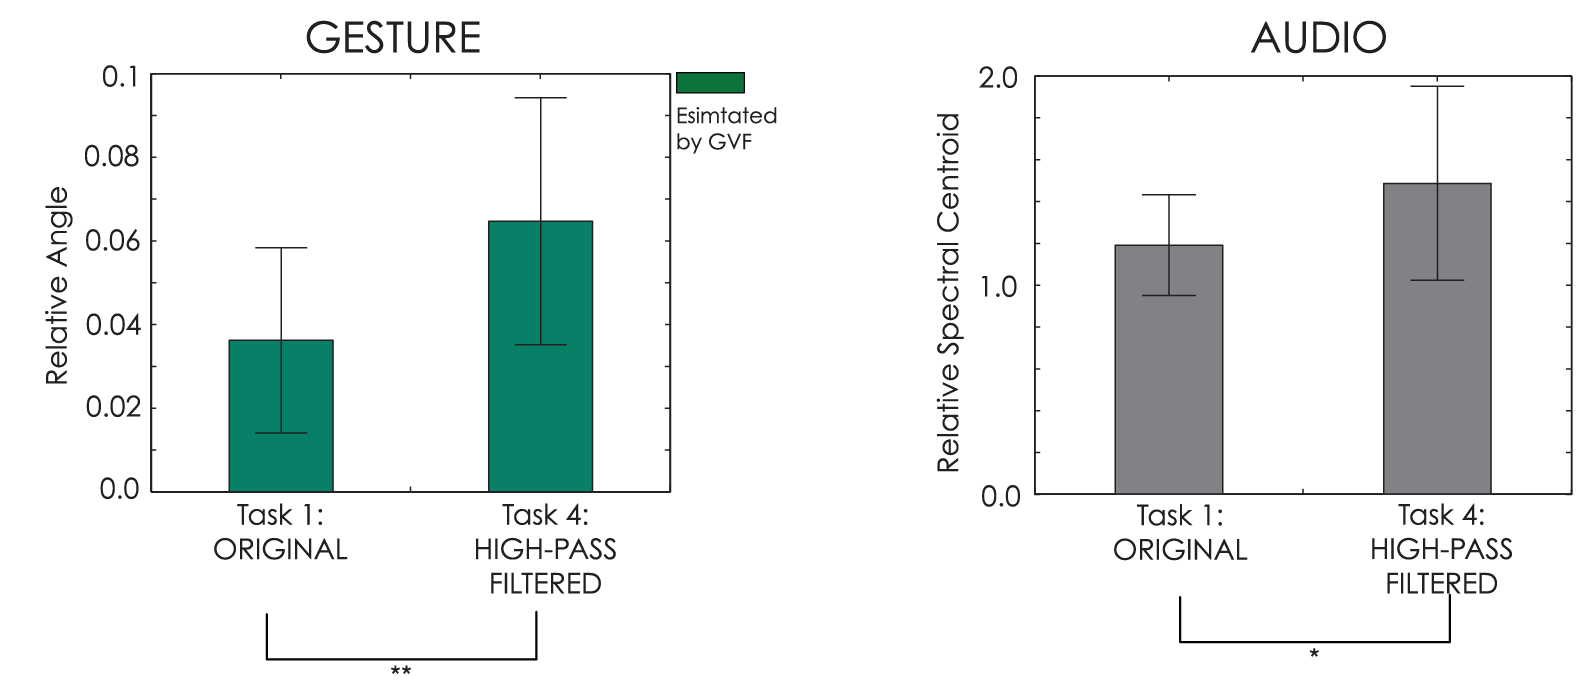
\includegraphics[width=0.7\linewidth]{../Bilder/Fig15}
\caption{Ergebnisse von Aufgabe 4 im Vergleich mit 1}
\label{fig:Fig15}
\end{figure}

Obwohl mangels Referenzpunkte für diese Aufgabe keine Nachanalyse der Geste möglich war, wurde vom Algorithmus eine Drehung der Geste gemeldet, was sich in der Anwendung des Hochpassfilters deutlich macht.

\subsection{kontinuierliche Änderung einer Eigenschaft}
\begin{figure}
\centering
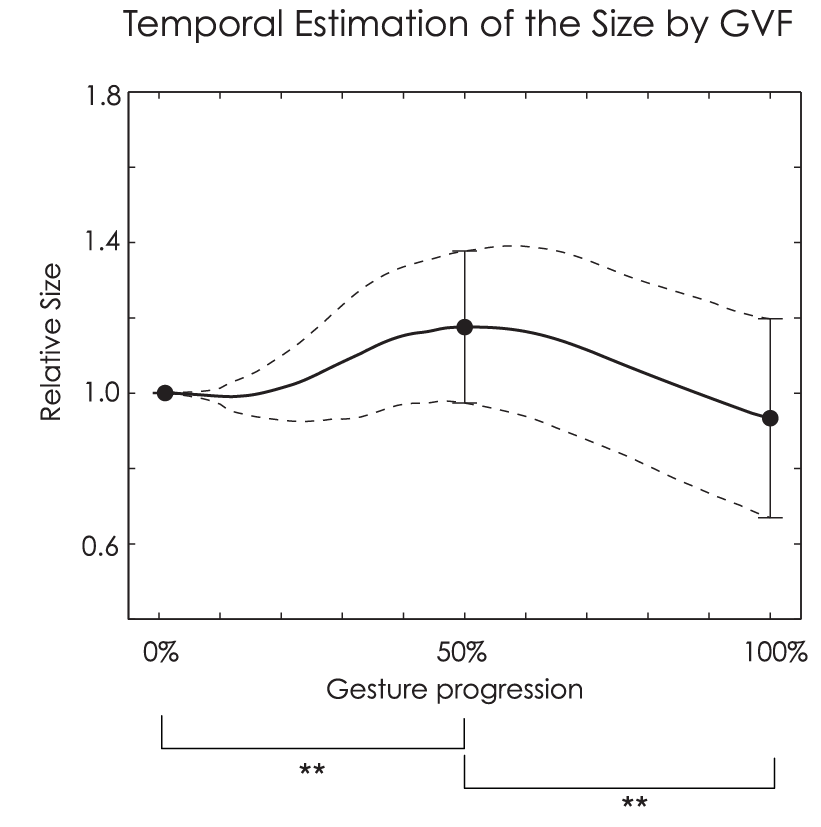
\includegraphics[width=0.7\linewidth]{../Bilder/Fig16}
\caption{Geschätzte Geschwindigkeit im Verlauf der Geste}
\label{fig:Fig16}
\end{figure}

In Aufgabe 5 wurde von den Teilnehmern verlangt, den Ton zumächst laut zu spielen und während der Ausführung der Geste leiser zu werden. Wenn man die geschätzten Werte bei $0$, $50$ und $100\%$ Fortschritt betrachtet, so wird deutlich, dass die Größe der Geste zunächst zunimmt und in der zweiten Hälfte wieder fällt. Somit wird deutlich, dass die Teilnehmer die Aufgabe erfolgreich bewältigt haben.

\subsection{Änderung zweier Eigenschaften}
\begin{figure}
\centering
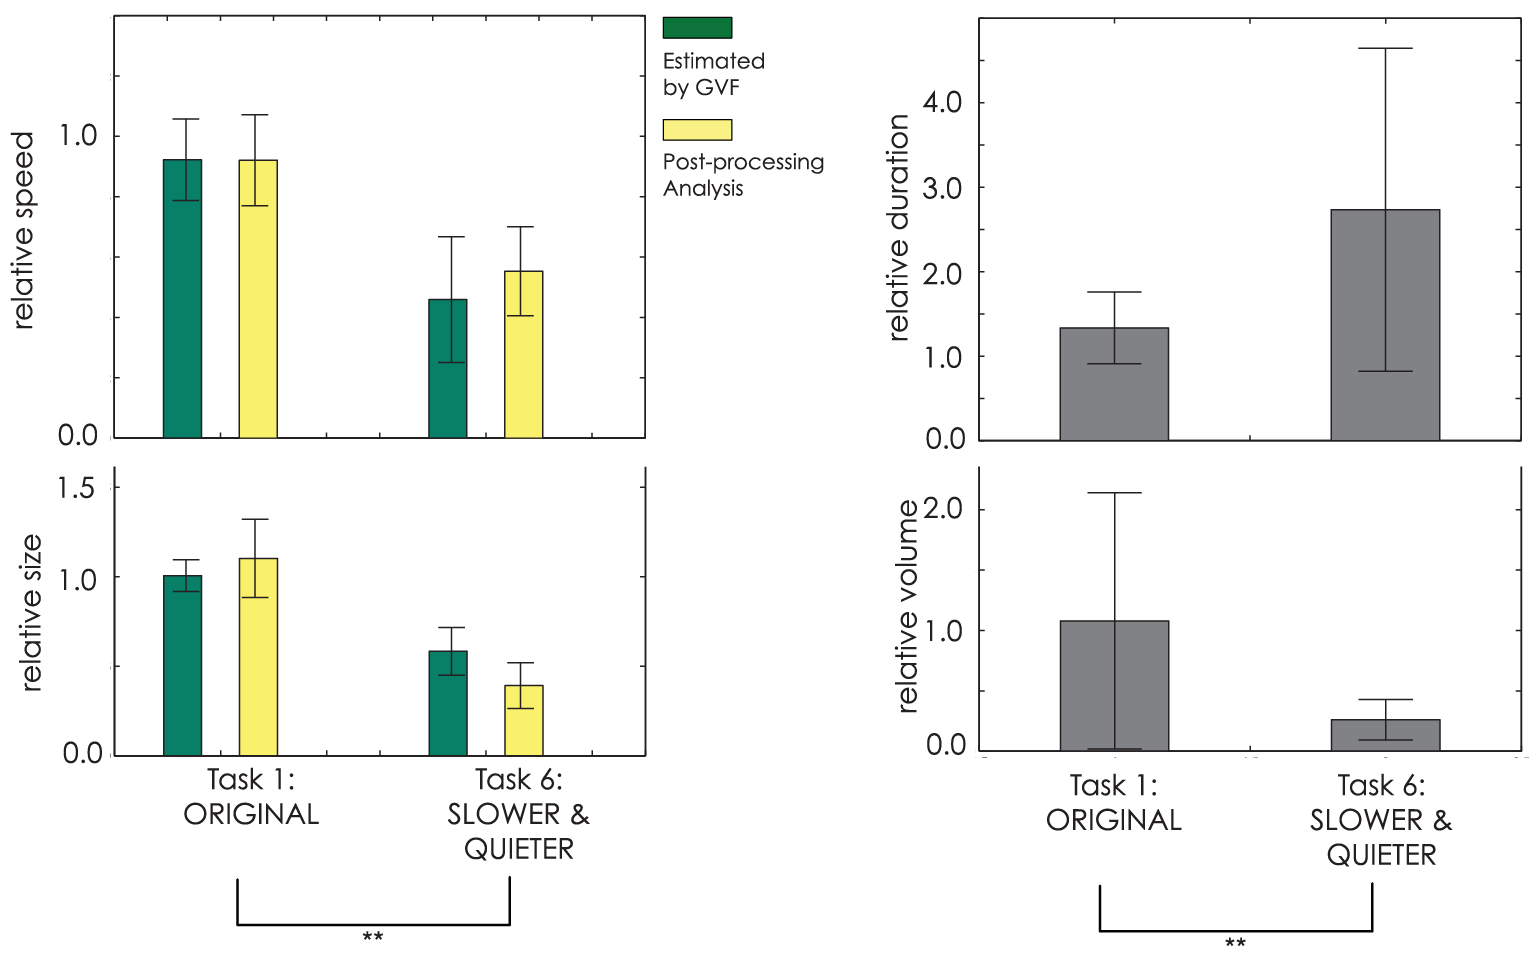
\includegraphics[width=0.7\linewidth]{../Bilder/Fig17}
\caption{Ergebnisse von Aufgabe 6 im Vergleich mit 1}
\label{fig:Fig17}
\end{figure}
\begin{figure}
\centering
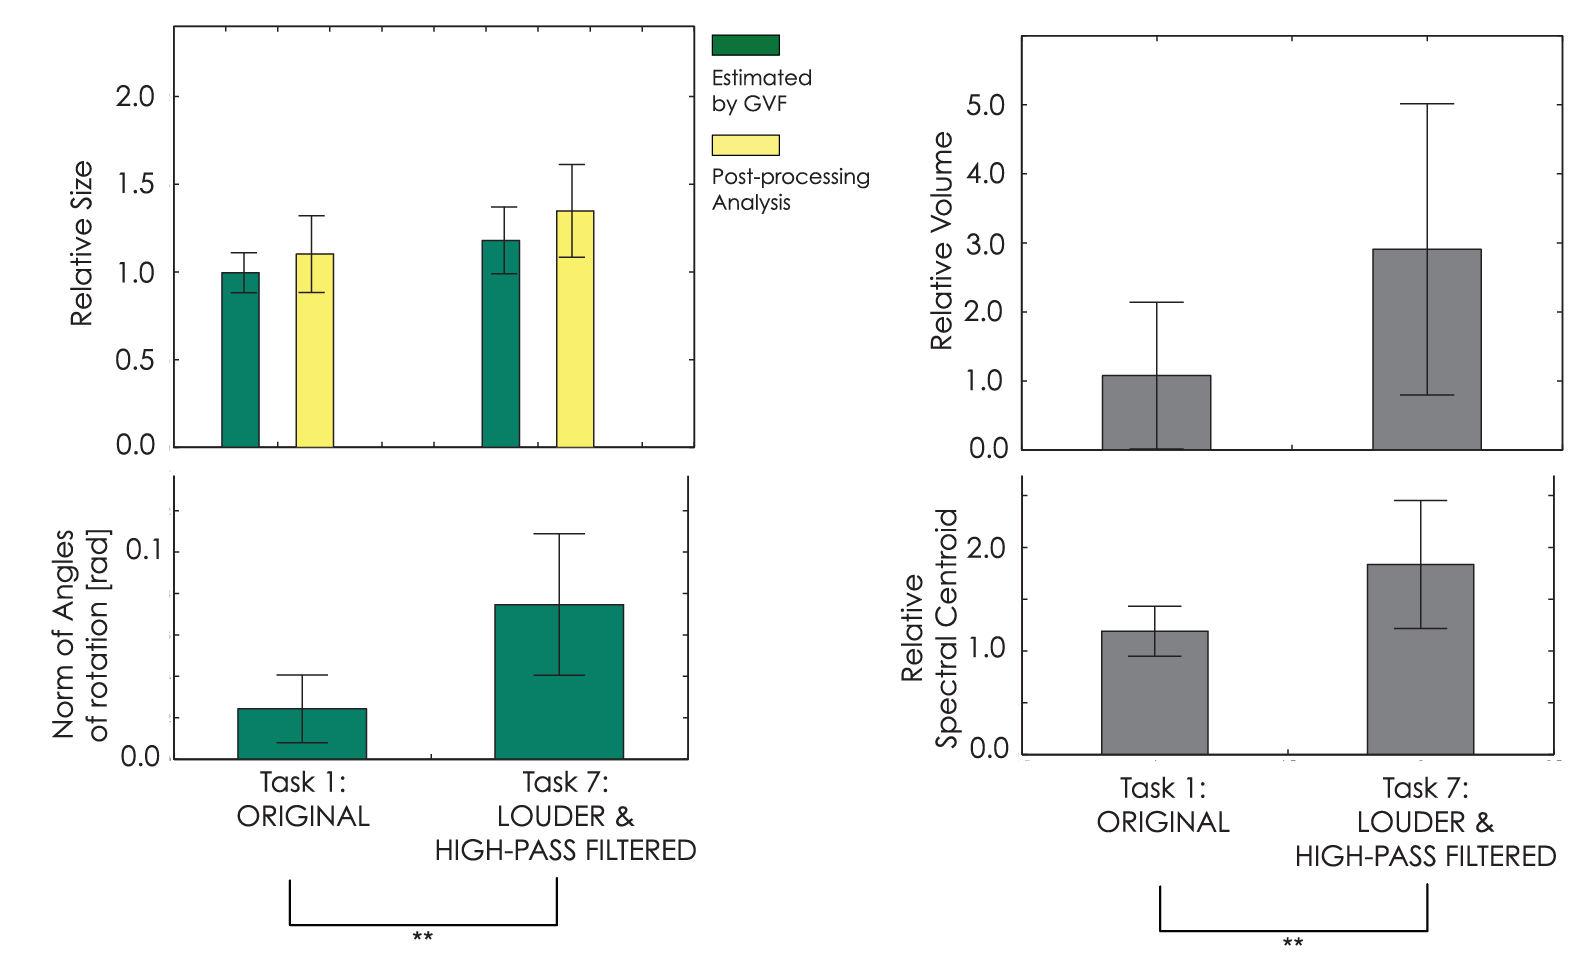
\includegraphics[width=0.7\linewidth]{../Bilder/Fig18}
\caption{Ergebnisse von Aufgabe 7 im Vergleich mit 1}
\label{fig:Fig18}
\end{figure}

In den Aufgaben 6 und 7 wurde von den Teilnehmern verlangt, den Ton lauter und langsamer, bzw. leiser mit Hochpassfilter zu spielen. Wie aus den Abbildungen \ref{fig:Fig17} und \ref{fig:Fig18} deutlich wird, ist dies den Teilnehmern gelungen.

\subsection{Beobachtungen der Nutzerstudie}
Insgesamt haben die Teilnehmer die ihnen gestellten Aufgaben verstanden, und haben es geschafft, die verlangten Ergebnnisse zu erzielen. Die Analyse der wiedergegebenen Töne und abgeschätzten Variationen macht deutlich, dass der Algorithmus die Gesten richtig abschätzt.



 
\bibliography{paper}
\bibliographystyle{plain}
\end{document}
